\documentclass[11pt]{beamer}

\usetheme[progressbar=frametitle]{metropolis}
\usepackage{appendixnumberbeamer}
\usepackage{pgfpages}
%\setbeameroption{show notes on second screen}



\newcommand{\link}[3][mLightBrown]{\href{#2}{\color{#1}{#3}}}%

\newcommand{\questionslide}[0]{
\section[Your questions]{Time for your questions}
{\setbeamercolor{palette primary}{fg=black, bg=yellow} % bg=peppermint
\begin{frame}[standout]
    \raggedright
  Any questions? \\ \vspace{1cm}
  \raggedleft
  \dots Remember -- this is a safe space! Every question is useful!
\end{frame}
}}

\newenvironment{rcases}
  {\left.\begin{aligned}}
  {\end{aligned}\right\rbrace}

\usepackage{pgfopts}

\newenvironment{rcasesx}
  {\left.\begin{aligned}}
  {\end{aligned}\right.}


\setbeamercolor{block title alerted}{%
    use={block title, alerted text},
    bg=yellow,
    fg=black
}




\definecolor{peppermint}{RGB}{75, 161, 115}
\definecolor{TolLightBlue}{HTML}{88CCEE}
\definecolor{RedViolet}{HTML}{A1246B}
\definecolor{Salmon}{HTML}{F69289}


\setbeamercolor{alerted text}{fg=peppermint , bg= black}

\usepackage{booktabs}
\usepackage[scale=2]{ccicons}

\usepackage{pgfplots}
\usepgfplotslibrary{dateplot}

\makeatletter 
\def\beamer@framenotesbegin{% at beginning of slide
    \usebeamercolor[fg]{normal text}
    \gdef\beamer@noteitems{}% 
    \gdef\beamer@notes{}% 
}
\makeatother


\usepackage{xspace}
\newcommand{\themename}{\textbf{\textsc{metropolis}}\xspace}

\title{Bias}
\subtitle{Econ 140 Spring 2025, Section 3}
% \date{\today}
\date{}
\author{Jonathan Old}

\institute{ \link{https://docs.google.com/document/d/1aJLqXpJkgN0fKDtEwYge8xHyxrnHQ2PGlsx9xOsmq-Y/}{Syllabus/OH} \hspace{0.2cm} \link{https://bcourses.berkeley.edu/courses/1542035/files/folder/Sections/Jonathan\%20(Sections\%20110\%2C\%20112)}{bCourses}  \hspace{0.2cm} \link{https://jonathanold.github.io/teaching.html}{Website}  \hspace{0.2cm} \link{https://forms.gle/HuV4DZCKyG5nTbVu6}{Feedback form (\textbf{Always open})} \hspace{0.2cm} \link{https://posit.co/downloads/}{RStudio}}
% \titlegraphic{\hfill\includegraphics[height=1.5cm]{logo.pdf}}

\usepackage{hyperref}

\begin{document}


\maketitle

\begin{frame}{Roadmap}
  \setbeamertemplate{section in toc}[sections numbered]
  \tableofcontents%[hideallsubsections]
\end{frame}




\questionslide





\section{Recap}


\begin{frame}{Recap: Regression}
    See on blackboard
\end{frame}




\begin{frame}{Recap: Selection bias}
We saw that whenever we do a difference-in-means comparison (or a regression), we get:\\
\vspace{0.4cm}
 \begin{columns}
          \column{0.38\linewidth}
             \centering
             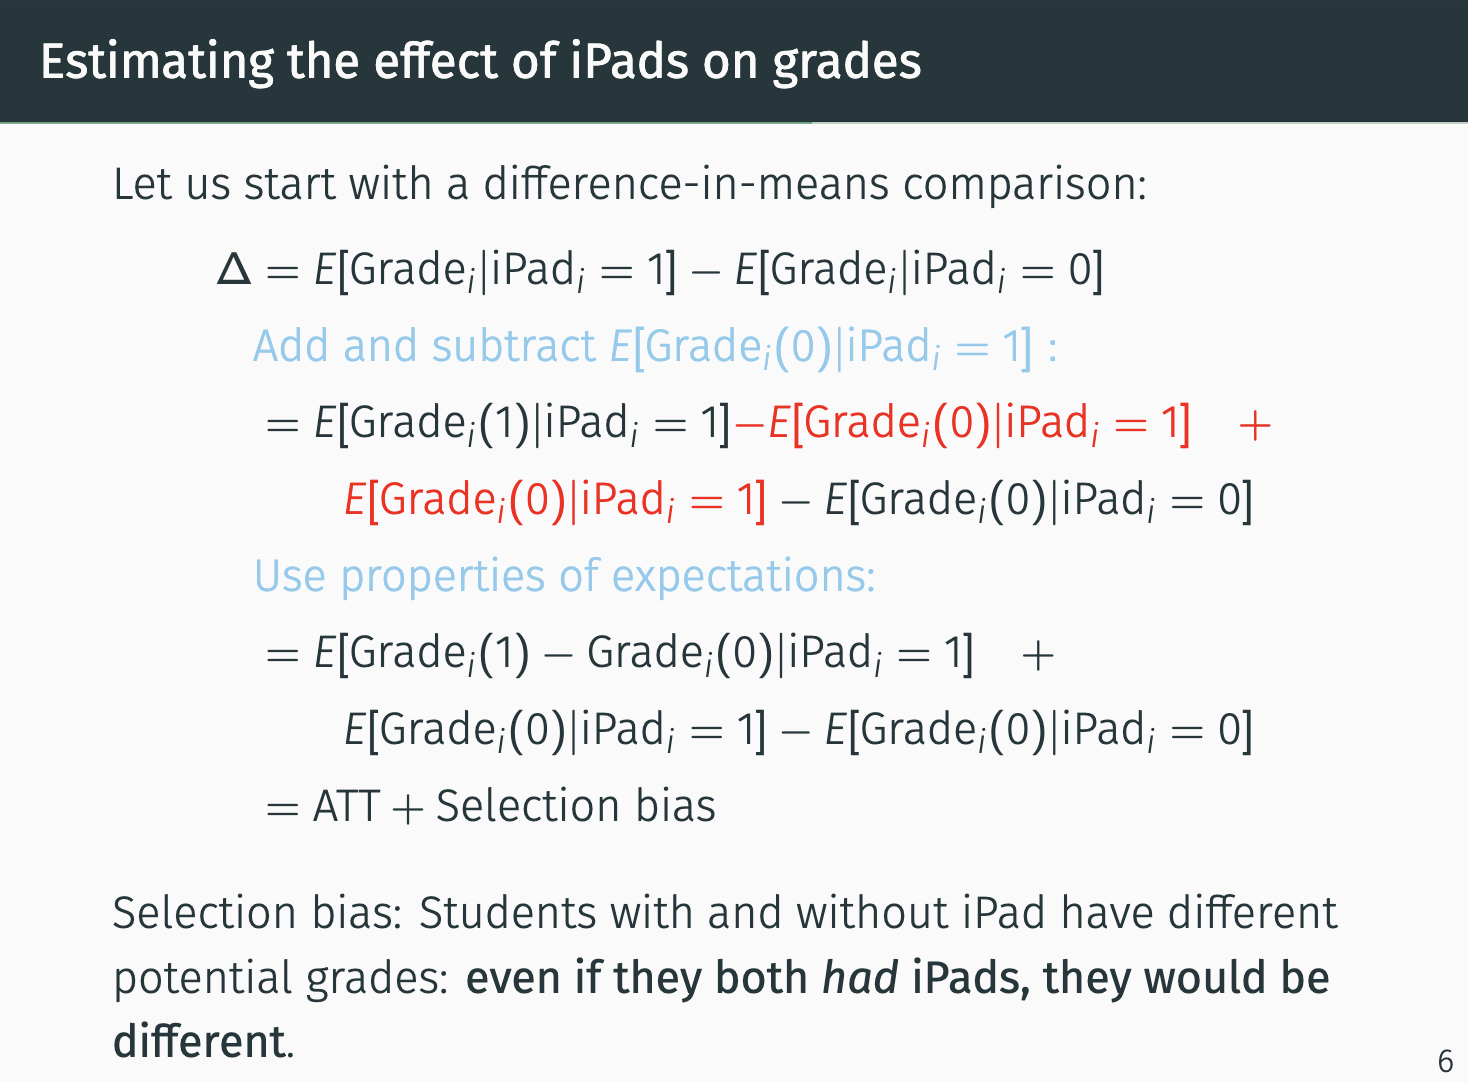
\includegraphics[width=4cm]{figures/s3_selectionbias.png}
           \column{0.58\linewidth}
            {\huge \centering{ 
            Causal Effect \\
            \textbf{{\color{red} +}} \\
            Selection Bias \\ }}
         \end{columns} 
\vspace{0.6cm}
\begin{itemize}
    \item We cannot observe them - so we can never be sure!
 \item Econometrics is all about uncertainty. You can \alert{always} state that there are different possibilities and you cannot know for sure
\end{itemize}
         
\end{frame}







\begin{frame}{Recap: How to think about Selection Bias}
    \begin{figure}
        \centering
        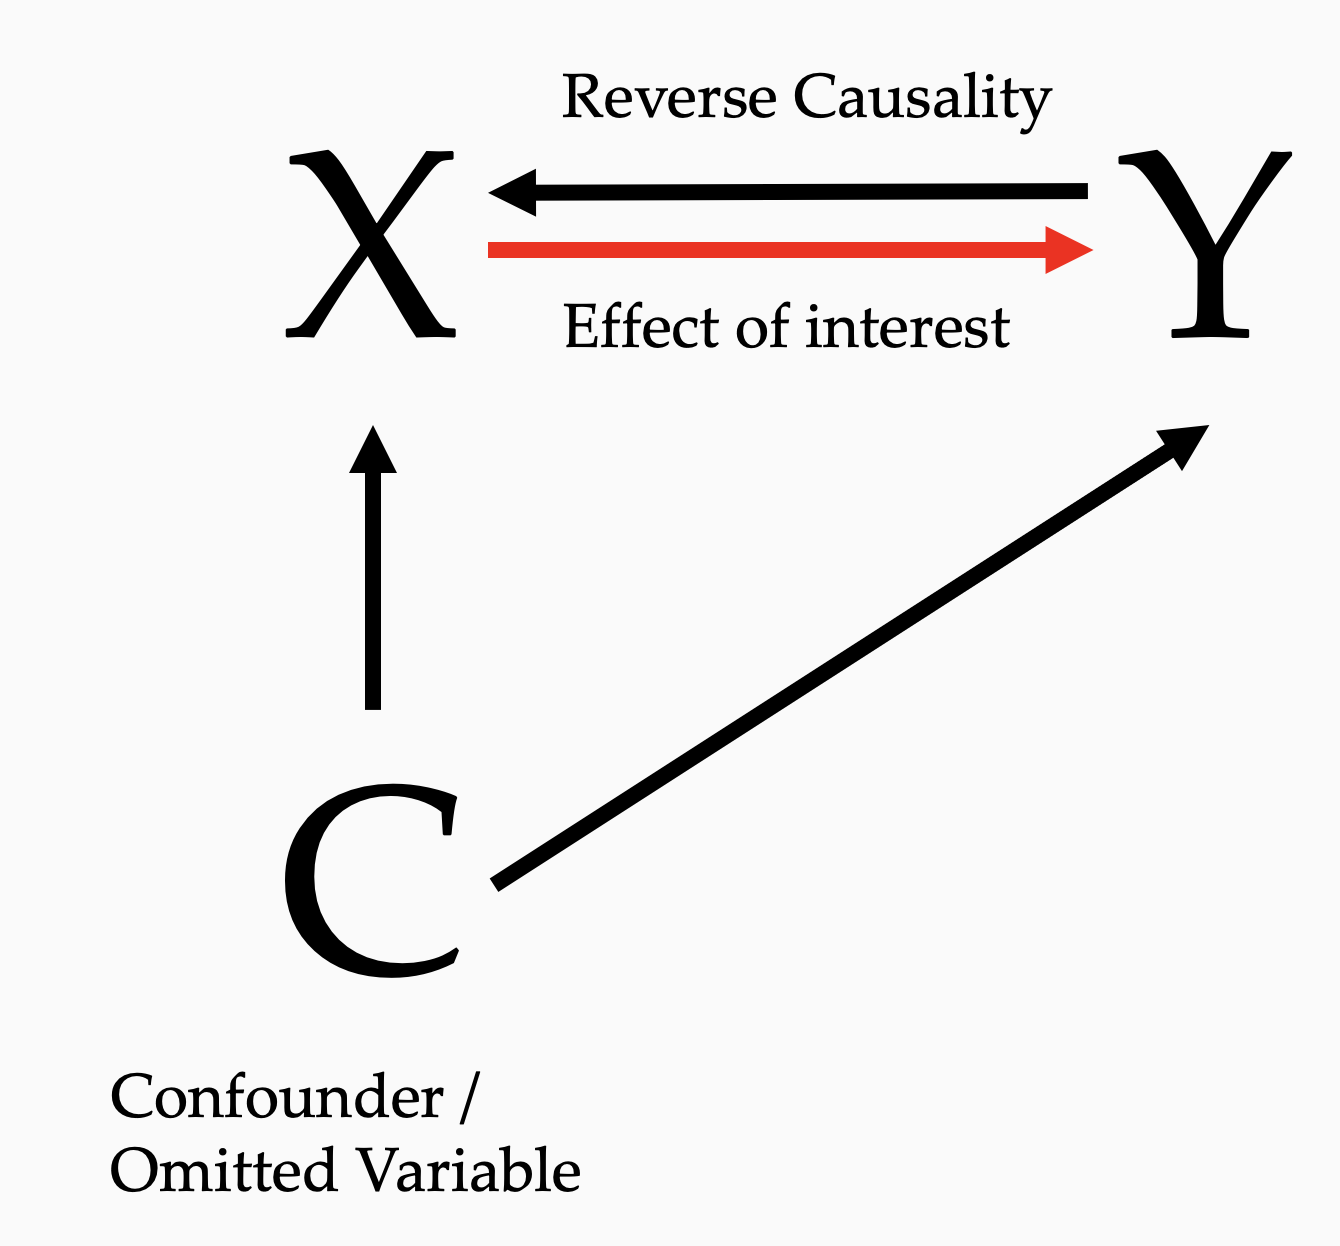
\includegraphics[width=0.5\textwidth]{DAGs/selectionbias.png}
        \caption{Selection bias}
        \label{fig:selectionbias}
    \end{figure}
\end{frame}




\section{Selection bias in action: Omitted Variable Bias}







\begin{frame}{The most important slide of this course (until the midterm)}
Let $Y_i$ be the outcome variable, $X_i$ our regressor of interest, $W$ a series of control variables, and $Z_i$ the "omitted" variable.
\begin{align*}
   \text{[Long regression]} \quad Y_i &= \alpha_L + {\color{peppermint}\beta_L} X_i + {\color{RedViolet}\lambda}Z_i +  W\beta_{WL}  + e_i^S \\
   \text{[Short regression]} \quad Y_i &= \alpha_S + {\color{gray}\beta_S} X_i  + W\beta_{WS}  +e_i^L \\
   \text{[Auxiliary regression]} \quad Z_i &= \pi_0 +  {\color{Salmon}\pi_
1} X_i + W\pi_{WP}  +v_i 
\end{align*}
    Then, the \textbf{Omitted variable bias formula} states that:
\begin{align*}
   \underbrace{\vphantom{ \left(\frac{a^{0.3}}{b}\right) }{\color{gray}\beta_S}}_{\text{Short =}} = \underbrace{\vphantom{ \left(\frac{a^{0.3}}{b}\right) }{\color{peppermint}\beta_L}}_{\text{Long }+} + \underbrace{\vphantom{ \left(\frac{a^{0.3}}{b}\right) }{\color{RedViolet} \lambda}}_{\text{Omitted } \times} \cdot \underbrace{\vphantom{ \left(\frac{a^{0.3}}{b}\right) }{\color{Salmon}\pi_{1}}}_{\text{Included}}
\end{align*}


The OVB formula describes what happens to our coefficient of interest, $\beta$, as we include one additional variable $Z$ in the regression. We call ${\color{RedViolet} \lambda} {\color{Salmon}\pi_{1}
}$ the \textbf{omitted variable bias}. 
Direction of bias: multiply our guesses for the signs of ${\color{RedViolet} \lambda}$ and ${\color{Salmon}\pi_1}$.
\end{frame}




\begin{frame}{Control variables}
Control variables are additional variables (or covariates) \textbf{included in a regression}. We do this for \textbf{various reasons} (in decreasing order of importance):
\begin{itemize}
    \item To remove selection bias / omitted variable bias
    \item To increase precision of our estimates
    \item To know about the (conditional/partial) correlation of other variables
    \item To better predict the outcome
\end{itemize}

\alert{Let's see \textit{\href{https://datahub.berkeley.edu/user/jonathan\_old/lab/tree/ECON-140-FA24-RDE/Sections/Jonathan/Omitted\%20Variables\%20Bias\%20Example.ipynb}{graphically}} how control variables work!}
\end{frame}




\questionslide 






\section{Inference and hypothesis testing}



\begin{frame}{Hypothesis testing}
We need a few ingredients:

\begin{itemize}
    \item \alert{Random variables}: Our estimator is a random variable (randomly drawn from population) 
    \item \alert{Standard error}: Random variables have a standard deviation, estimators have standard errors. This quantifies their uncertainty 
    \item \alert{Statistics}: The two keywords are the law of large numbers and the central limit theorem: The sum/mean of many random variables will follow normal distribution 
    \item \alert{For hypothesis test}: null and alternative hypothesis. 
    \item We assume that the null hypothesis is true and then see \alert{how plausible results are}, given the null is true. 
    \item If they are implausible -- we \alert{reject the null hypothesis}! Otherwise: Fail to reject.
    \end{itemize}
\end{frame}


\begin{frame}{It's all connected}

   \begin{figure}
        \centering
        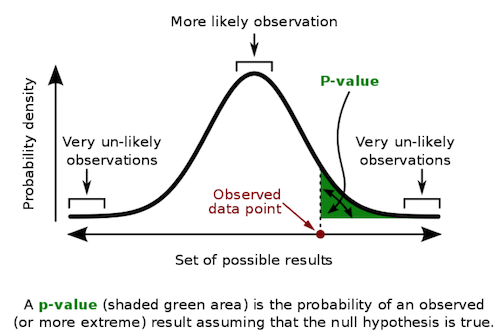
\includegraphics[width=0.8\textwidth]{figures/hypothesis testing/p_value.png}
        
    \end{figure}


\end{frame}



\begin{frame}{Hypothesis testing mini-cheatsheet}
\vspace{-0.2cm}
\LARGE
\begin{align*}
    \left| \frac{\hat{\beta}}{\operatorname{SE}(\hat{\beta})} \right| &\geq 1.96 \\ 
    \Leftrightarrow | \operatorname{t-stat}| &\geq 1.96 \\  \Leftrightarrow \operatorname{p-value} &\leq 0.05 \\
    \Leftrightarrow 0 &\notin \text{CI}
\end{align*}
\\
\normalsize \alert{If you are testing the null hypothesis $H_0$: $\beta = 0$ (against the alternative hypothesis $H_0$: $\beta \neq 0$), then all of these are equivalent, and you can use any of these.}

\end{frame}







\section{Exam practice}

\begin{frame}{Practice exam question: 1a)}

   \small{The Ministry of Truth is interested in a rumour that \textbf{air pollution could impact mental health}. One of the most harmful pollutants is fine particulate matter PM2.5, which comes from operations that involve the burning of fuels such as wood, oil, coal, etc. A research team is sent to investigate the rumour. The team \textbf{randomly} selects and surveys 19,920 people across 71 districts of the country. The key variable, Exposure $E_i$, is a \textbf{dummy variable} equal to 1 if the individual $i$ is exposed to a large amount of PM2.5 in the last 24 hours, and 0 otherwise. The team also conducts a standardised questionnaire to record \textbf{depressive symptoms} in the last month, called the Kessler Psychological Distress scale (K6). The questionnaire results in a score, Depression$_i$, that ranges from 0 to 24; and the higher the score, the more severe the depressive symptoms for individual $i$. The variable has a sample average of 2.96. \textbf{Running regressions with Depression D$_i$ as  the dependent variable, you obtain the following results}:
}
    
\end{frame}



\begin{frame}{Practice exam question: 1a)}

\footnotesize
Dependent variable: Depression $_i$

\begin{tabular}{lccc}
\toprule
\textbf{Regressor}               & \textbf{$(1)$}       & $(2)$ & $(3)$                         \\
\midrule
Exposure $_i$                    & $0.834$              & $0.614$                                                   & $0.554$                       \\
                                 & $(0.032)$            & $(0.045)$                                                 & $(0.042)$                     \\
Exposure $_i \times$ Female $_i$ &                      & $0.065$                                                   &                               \\
                                 &                      & $(0.024)$                                                 &                               \\
Female $_i$                      &                      & $-0.739$                                                  & $-0.825$                      \\
                                 &                      & $(0.036)$                                                 & $(0.066)$                     \\
Age$_{i}$                        &                      &                                                           & $0.452$                       \\
                                 &                      &                                                           & $(0.132)$                     \\
Age$_i^2$    &                      &                                                           & $0.524$                       \\
                                 & \multicolumn{1}{l}{} & \multicolumn{1}{l}{}                                      & \multicolumn{1}{l}{$(0.121)$} \\
                                 \bottomrule \\
\end{tabular}  \\

Notes: All estimations contain a constant term. Robust standard errors are in the parentheses. Age$_i$ is the age (years old) of individual $i$, and Age$_i^2$ is the square of Age$_i$.

\end{frame}




\begin{frame}{Practice Exam question: 1a)}
   \textbf{a)} Interpreting the coefficient in Column (1), a journalist, Katherine, claims: "Since participants are randomly selected, we can infer that exposure to a large amount of PM2.5 does cause depression." \\
\textbf{i.} Explain carefully why Katherine is wrong. Come up with two confounding variables, specifying the direction of bias(es) if there are any. Which assumption(s) would she need to impose for the causality claim to hold? \\
\textbf{ii.} What is the correct interpretation from Column (1) that Katherine should have made?
\end{frame}


\begin{frame}{(Detailed) Suggested Answer: 1a)}
\footnotesize{
\textbf{i.} \textbf{ Random selection is not the same thing as random assignment to treatment!} Survey respondents may be systematically different from each other in ways that are correlated with depression and pollution exposure. Therefore, the results from a regression can not be interpreted causally (and are biased). A priori, it is unclear in which direction the bias would go, but we could imagine that (\textbf{Only one explanation needed for exam}):\\
On rainy days, pollution is lower (-) and people may be reporting more depression symptoms (+), leading to downward bias.
More wealthy people choose to live in less polluted areas (-) and they may have less depression (e.g., better access to mental health resources) (-), leading to upward bias.\\

For the regression causality claim to hold, we need to assume that:
People exposed to pollution and those not exposed to pollution would have, on average, the same depression level, had they been exposed to the same level of pollution. In other words: \textbf{Both groups would have to have the same potential depression outcomes}.\\

\textbf{ii.} On average, people that were exposed to pollution had a 0.8 points higher score on the depression scale. The difference between the two groups is significant at the 5\% level.
}
\end{frame}





\begin{frame}{Pratice Exam question: 1b)}
   \textbf{b)} Interpret column (2) of the regression table \\
\textbf{i.} A colleague notes the the coefficient on Female$_i$ is significant, and states: "The effect of being female on depression is significantly different from zero". Do you agree with the statement? Why or why not? \\
\textbf{ii.} How is pollution exposure related to depression, for men? And how for women?
\end{frame}



\begin{frame}{(Detailed) Suggested Answer: 1b)  }
\footnotesize{
\textbf{i.} \textbf{It is difficult to make such interpretations when interaction terms are involved.} Taking partial derivatives, the "effect" of being female is:
$$ \frac{\partial \text{Depression}_i}{\partial \text{Female}_i} = -0.739 + 0.065\cdot \text{Exposure}_i $$
We can do inference (and test significance) at Exposure$_i=0$ (just looking at the coefficient for female, $-0.739$ is significant). We can also do it for any other level of exposure, but for that we also need to take the other coefficient into account and cannot just use the table.\\
\textbf{Comment 1: Less relevant for the exam, but important to be aware of!} \\
\textbf{Comment 2: We can always do inference on the interaction term, which is significant here!} 

\textbf{ii.} Taking partial derivatives, the "effect" of pollution exposure is:
$$ \frac{\partial \text{Depression}_i}{\partial \text{Exposure}_i} = 0.614 + 0.065\cdot \text{Female}_i $$
Hence, the "effect" for Males is $0.614$ and the "effect" for Females is larger ($0.614+0.065 = 0.779$). The effect of pollution is also \textbf{signficantly} larger than for men, because the coefficient on the interaction term is significantly different from zero.
}
\end{frame}


\begin{frame}
If time permits: Practice exam question, \href{https://drive.google.com/drive/u/4/folders/1-cQBZhZluOgRleSDZocxRj2OYfL8uOmj}{midterm 2022}.
\end{frame}



\end{document}
